\section{Subroutines and Stack}

\begin{concept}{Subroutine Basics}\\
Key elements of subroutines:
\begin{itemize}
  \item Label to identify subroutine entry point
  \item Return instruction (BX LR) to exit
  \item Proper register management
\end{itemize}
\end{concept}

\begin{example2}{Simple Subroutine}
Multiply by 3 implementation:
\begin{lstlisting}[language=armasm, style=basesmol]
MulBy3  MOV     R4, R0      ; Save input value
        LSLS    R0, #1      ; Multiply by 2
        ADD     R0, R4      ; Add original value
        BX      LR          ; Return
\end{lstlisting}
\end{example2}

\begin{definition}{Stack Operations}\\
Stack characteristics:
\begin{itemize}
  \item \textbf{Stack Area}: Continuous RAM section
  \item \textbf{Stack Pointer (SP)}: R13, points to last written value
  \item \textbf{Direction}: Full-descending (grows toward lower addresses)
  \item \textbf{Alignment}: Word-aligned (4 bytes)
  \item \textbf{Data Size}: 32-bit words only
\end{itemize}

Main operations:
\begin{itemize}
  \item \textbf{PUSH}: Decrements SP, then stores words
  \item \textbf{POP}: Loads words, then increments SP
\end{itemize}

Stack constraints:
\begin{itemize}
  \item Number of PUSH and POP operations must match
  \item SP must stay between stack-limit and stack-base
\end{itemize}

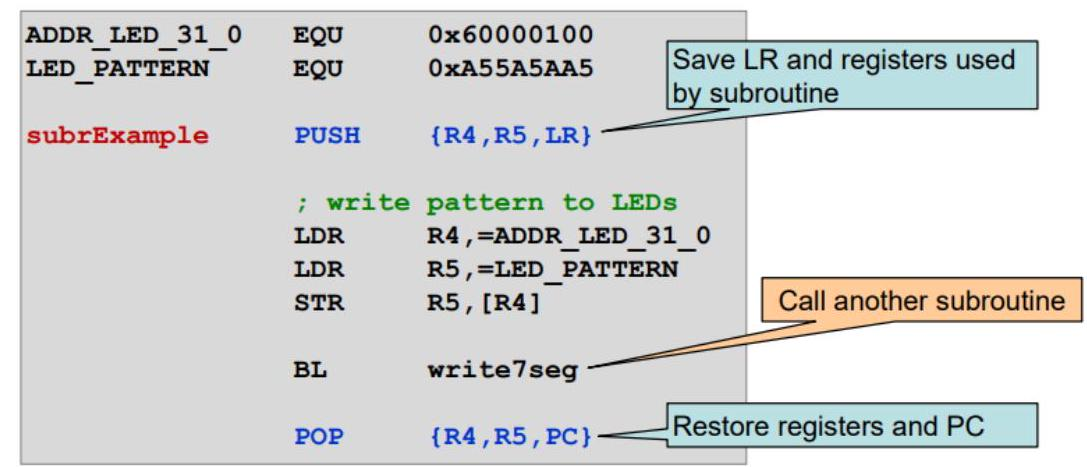
\includegraphics[width=\linewidth]{images/2024_12_29_79e6b22f503fb7b4f718g-08}
\end{definition}

\begin{example2}{Stack Operations Implementation}
PUSH implementation:
\begin{lstlisting}[language=armasm, style=basesmol]
    ; PUSH {R2,R3,R6}
    SUB     SP, SP, #12     ; Reserve stack space
    STR     R2, [SP]        ; Store R2
    STR     R3, [SP, #4]    ; Store R3
    STR     R6, [SP, #8]    ; Store R6
\end{lstlisting}

POP implementation:
\begin{lstlisting}[language=armasm, style=basesmol]
    ; POP {R2,R3,R6}
    LDR     R2, [SP]        ; Restore R2
    LDR     R3, [SP, #4]    ; Restore R3
    LDR     R6, [SP, #8]    ; Restore R6
    ADD     SP, SP, #12     ; Free stack space
\end{lstlisting}
\end{example2}

\begin{KR}{Using Subroutines and Stack}\\
Steps for implementing subroutines:
\begin{enumerate}
  \item Define subroutine entry point with label
  \item Save registers that will be modified
    \begin{itemize}
      \item Use PUSH at start
      \item Include LR if calling other subroutines
    \end{itemize}
  \item Implement subroutine logic
  \item Restore registers in reverse order
    \begin{itemize}
      \item Use POP before return
      \item Can return using POP {..., PC} if LR was saved
    \end{itemize}
  \item Return using BX LR if LR wasn't saved
\end{enumerate}
\end{KR}

\begin{remark}
Important considerations:
\begin{itemize}
  \item Always maintain stack alignment
  \item Match PUSH/POP pairs exactly
  \item Be careful with SP manipulation
  \item Consider nesting depth for stack space
\end{itemize}
\end{remark}